\documentclass[10pt,a4paper]{article}
\usepackage[latin1]{inputenc}
\usepackage{amsmath}
\usepackage{amsfonts}
\usepackage{amssymb}
\usepackage{makeidx}
\usepackage{graphicx}
\usepackage{titlesec}
\usepackage[left=2.00cm, right=2.00cm, top=2.00cm, bottom=2.00cm]{geometry}
\title {Ejercicio 1 de clase en LaTeX}
\author{F\'ernandez Barbosa Luis Antonio}
\date{Febrero 16 del 2023}
\begin{document}
	\maketitle
	Una escalera de 25 \emph{ft.} esta recargada con su base a 7 \emph{ft.} de la pared. Si la escalera se resbala y su base se aleja a 3 \emph{ft./s.}\ ¿Con qu\'e rapidez cae la escalera del lado de la pared?
	$$$$
	$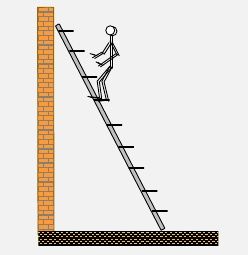
\includegraphics[width=8cm, height=5cm]{escalera.png}$
	$$$$
	$x=7\ \emph{ft.}$
	$$$$
	$\frac{dx}{dt}=3\ \frac{ft.}{s.}$ 
	$$$$
	$\frac{dy}{dt}=\ ?\ \frac{ft.}{s.}$
	$$$$
	$$f(x)=x^2 + y^2 = 25^2 \therefore y=\sqrt{625-49}=24$$
	$$f'(x)=2x\frac{dx}{dt}+2y\frac{dy}{dt}=0$$
	$$\frac{dy}{dt}=-\frac{2x\frac{dx}{dt}}{2y}$$
	$$\frac{dy}{dt}=-\frac{2*7*3}{2*24}=-\frac{42}{48}=-0.875$$
	$$\therefore$$
	$$\frac{dy}{dt}=0.875\ \frac{ft.}{s.}$$
	
\end{document}